\documentclass[9pt,a4paper,titlepage,oneside,mathserif,serif]{beamer}
\usepackage[latin1]{inputenc}
\usepackage{amsmath}
\usepackage{amsfonts}
\usepackage{amssymb}
\usepackage{graphicx}
%%Required for Felix 4-Faced SubFigures
\usepackage{subcaption}
\usepackage{mwe}

\author{Leonhard Applis}
\title{Edge Detection}
\subtitle{}
\institute{TH N�rnberg} % (optional)
\date{05.11.2018}
\subject{AvBildMed}

\usetheme{PaloAlto}
\usecolortheme{beaver}
\AtBeginSection[]
{
\begin{frame}
	\frametitle{Table of Contents}
	\tableofcontents[currentsection,currentsubsection]
\end{frame}
}

\begin{document}
\frame{\titlepage}
\section{What makes an Edge?}
\begin{frame}
	\frametitle{What makes an edge?}
	\begin{columns}
		\begin{column}{0.5\textwidth}
			\begin{figure}
				\centering
				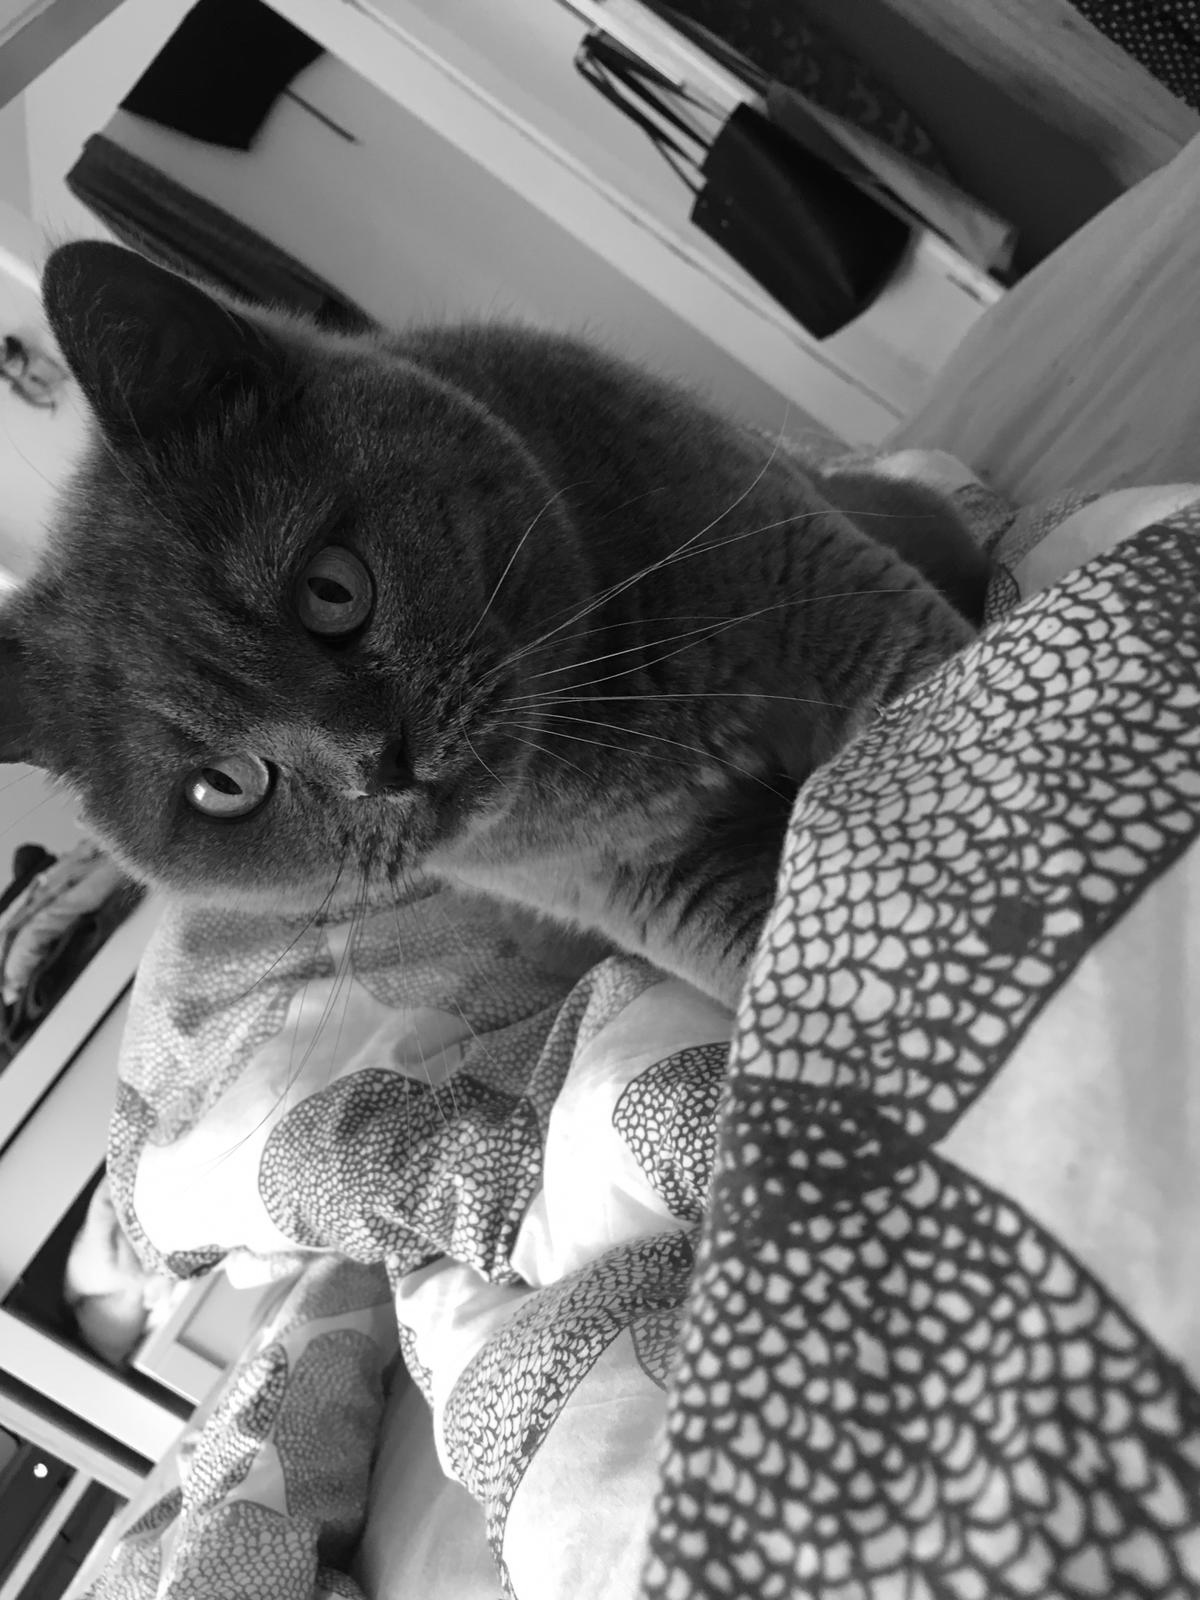
\includegraphics[width=0.8\linewidth]{images/Kadse}
				\caption[Felix]{Felix}
				\label{fig:kadse}
			\end{figure}
		\end{column}
		\begin{column}{0.5\textwidth} 
			\begin{center}
			\begin{figure}
				\centering
				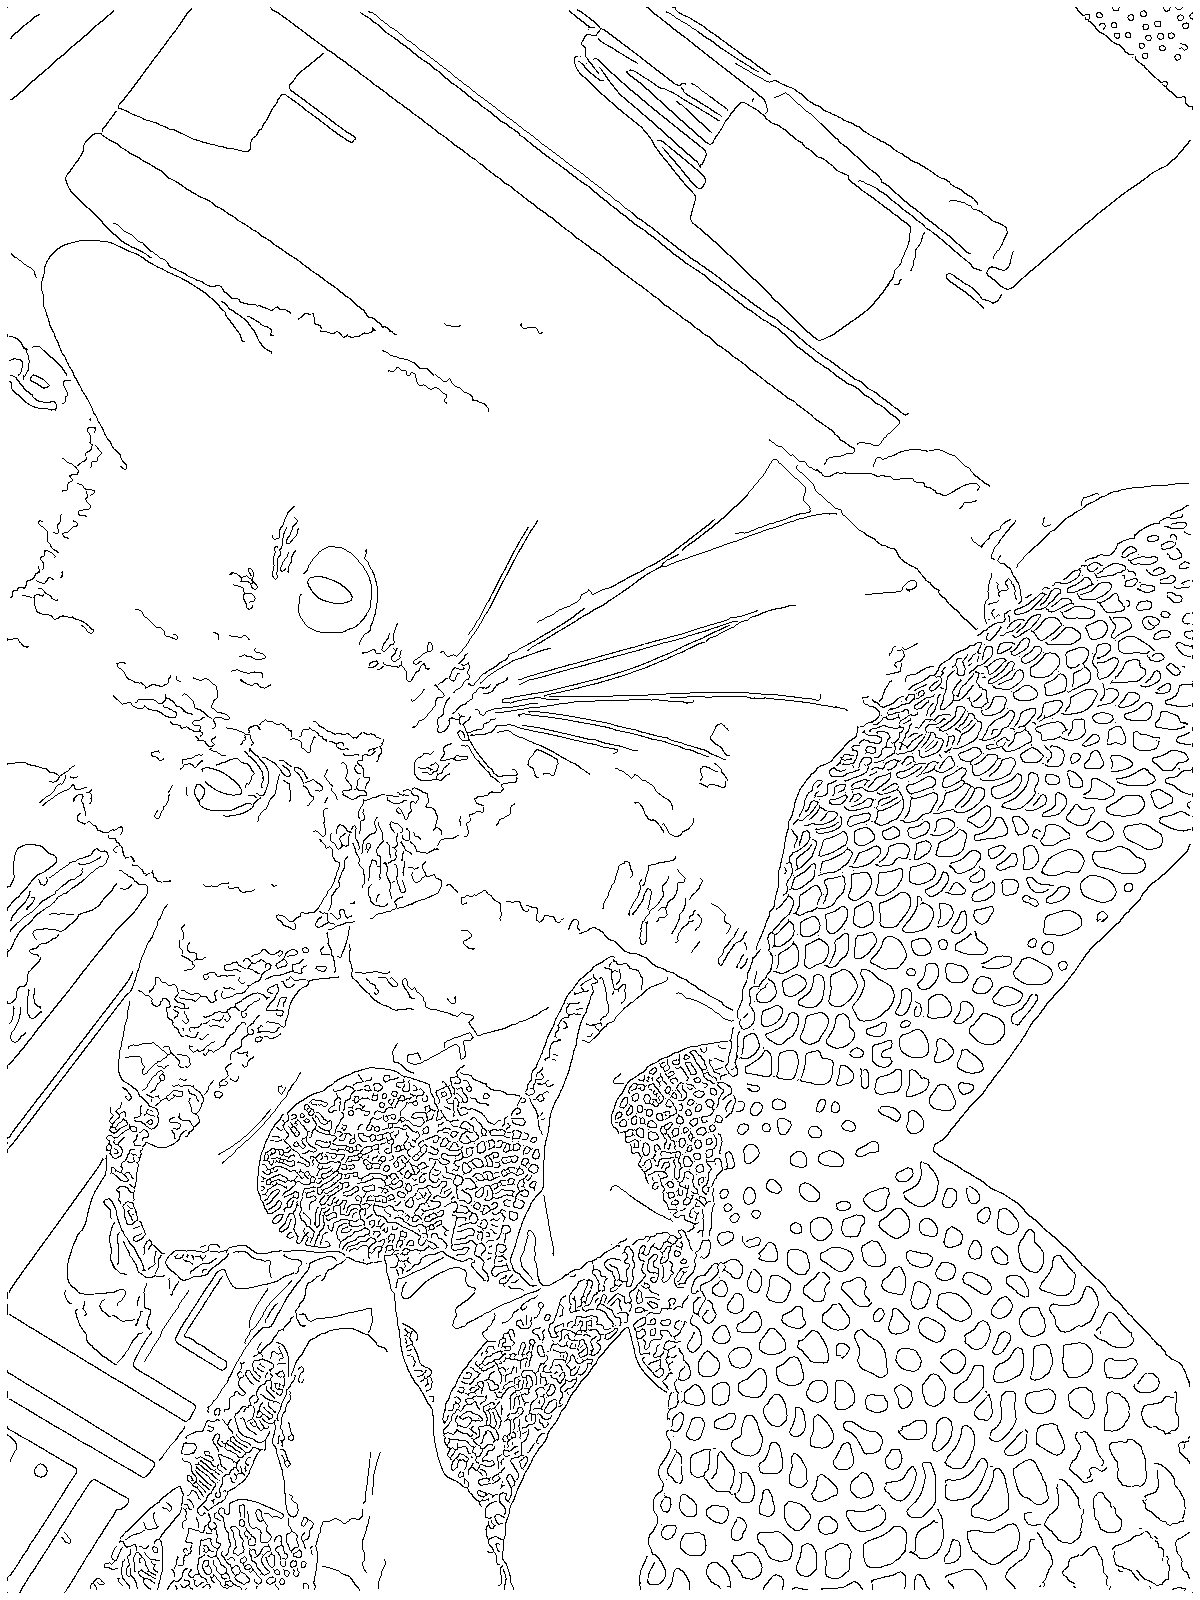
\includegraphics[width=0.8\linewidth]{images/KadseCanny}
				\caption[Felix's Edges]{Felix's Edges}
				\label{fig:kadseCanny}
			\end{figure}
			\end{center}
		\end{column}
	\end{columns}
\end{frame}
\subsection{Problems}
\begin{frame}
	\frametitle{Problem I: Contrast}
	\begin{columns}
		\begin{column}{0.5\textwidth}
			\begin{figure}
				\centering
				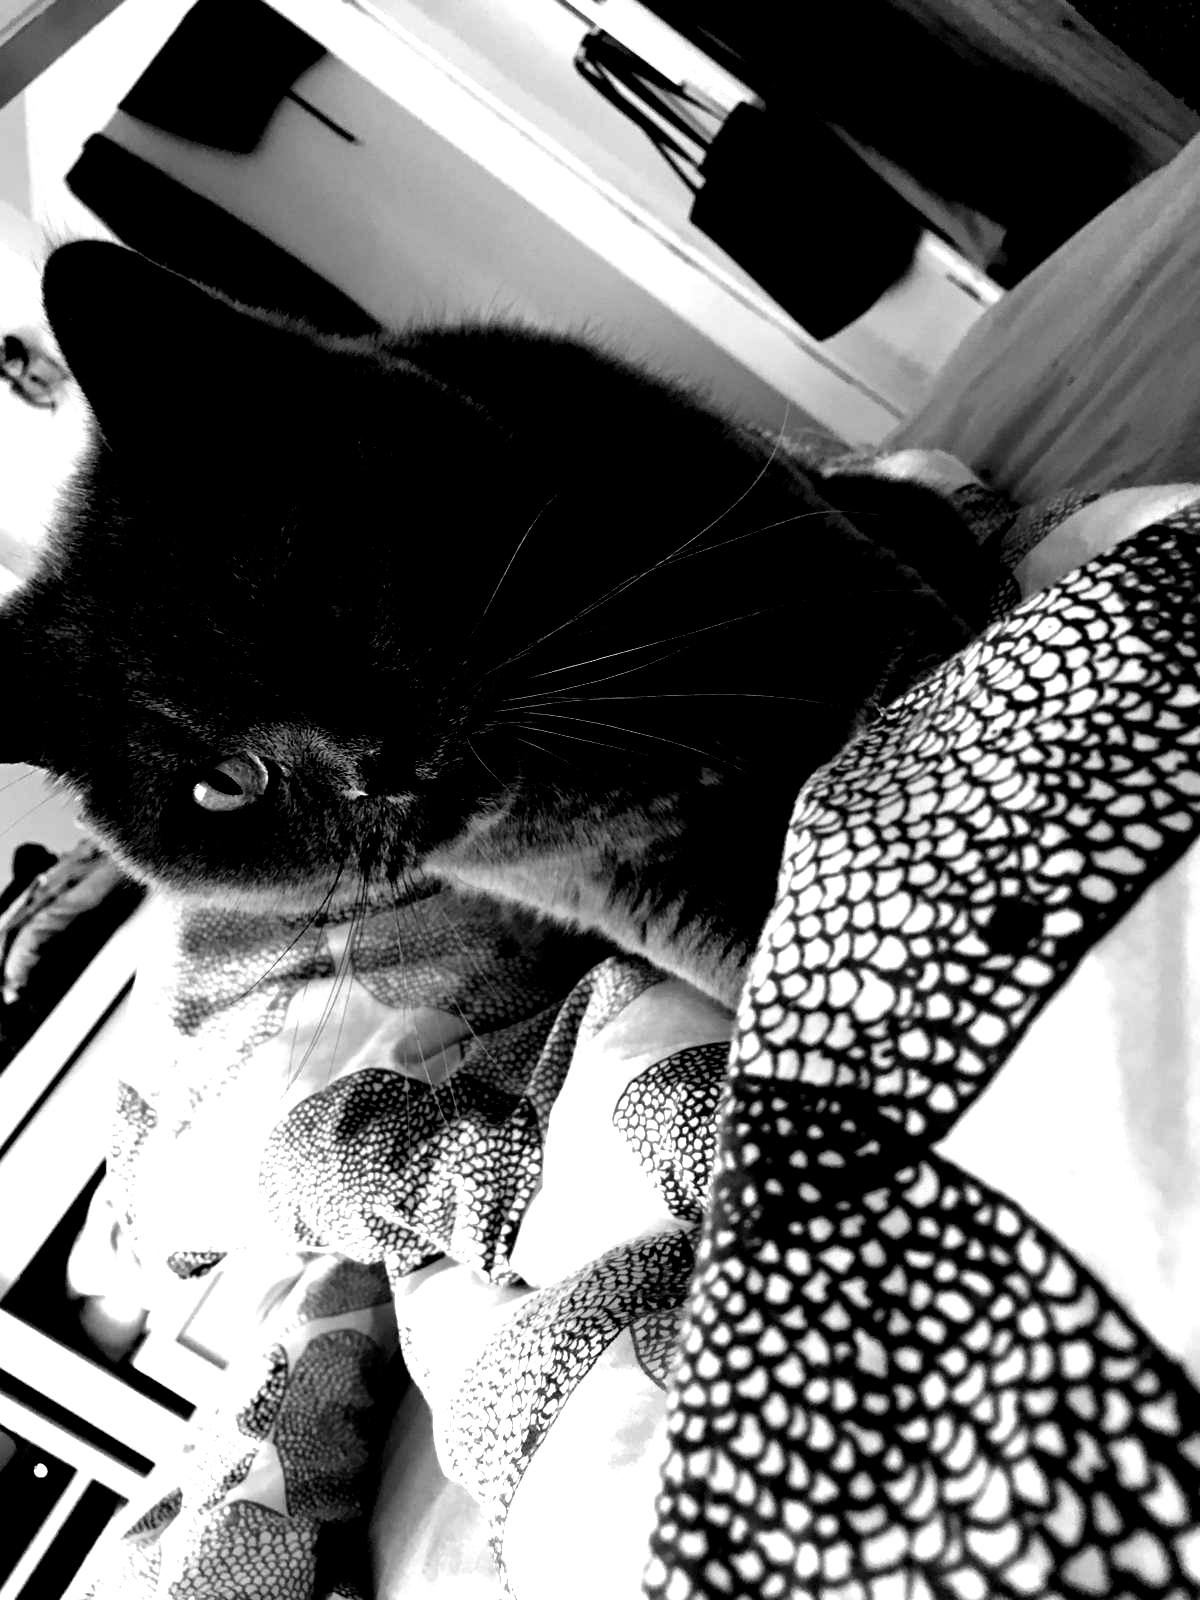
\includegraphics[width=0.8\linewidth]{images/KadseHighContrast}
				\caption[High Contrast Felix]{High Contrast Felix}
				\label{fig:HighContrast}
			\end{figure}
		\end{column}
		\begin{column}{0.5\textwidth} 
			\begin{center}
				\begin{figure}
					\centering
					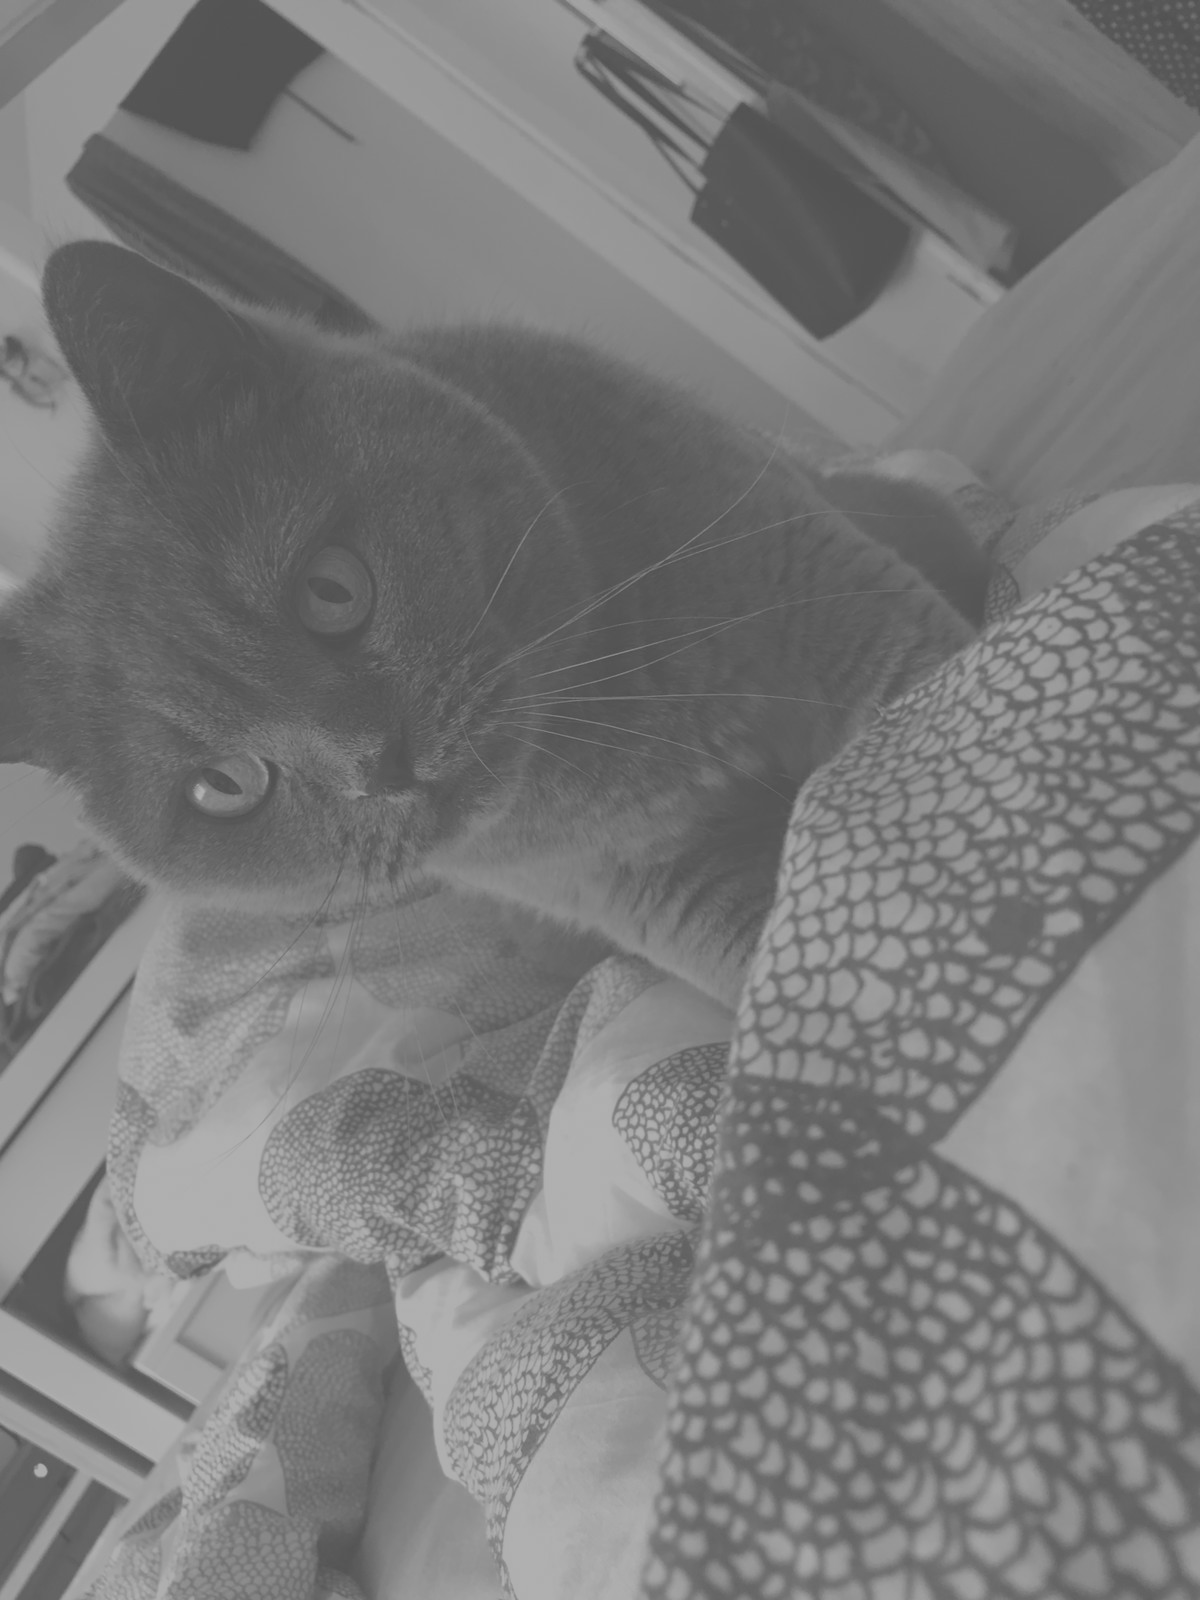
\includegraphics[width=0.8\linewidth]{images/KadseLowContrast}
					\caption[Low Contrast Felix]{Low Contrast Felix}
					\label{fig:LowContrast}
				\end{figure}
			\end{center}
		\end{column}
	\end{columns}
\end{frame}

\begin{frame}
	\frametitle{Problem II: Smoothness}
	\begin{center}
		\begin{figure}
			\centering
			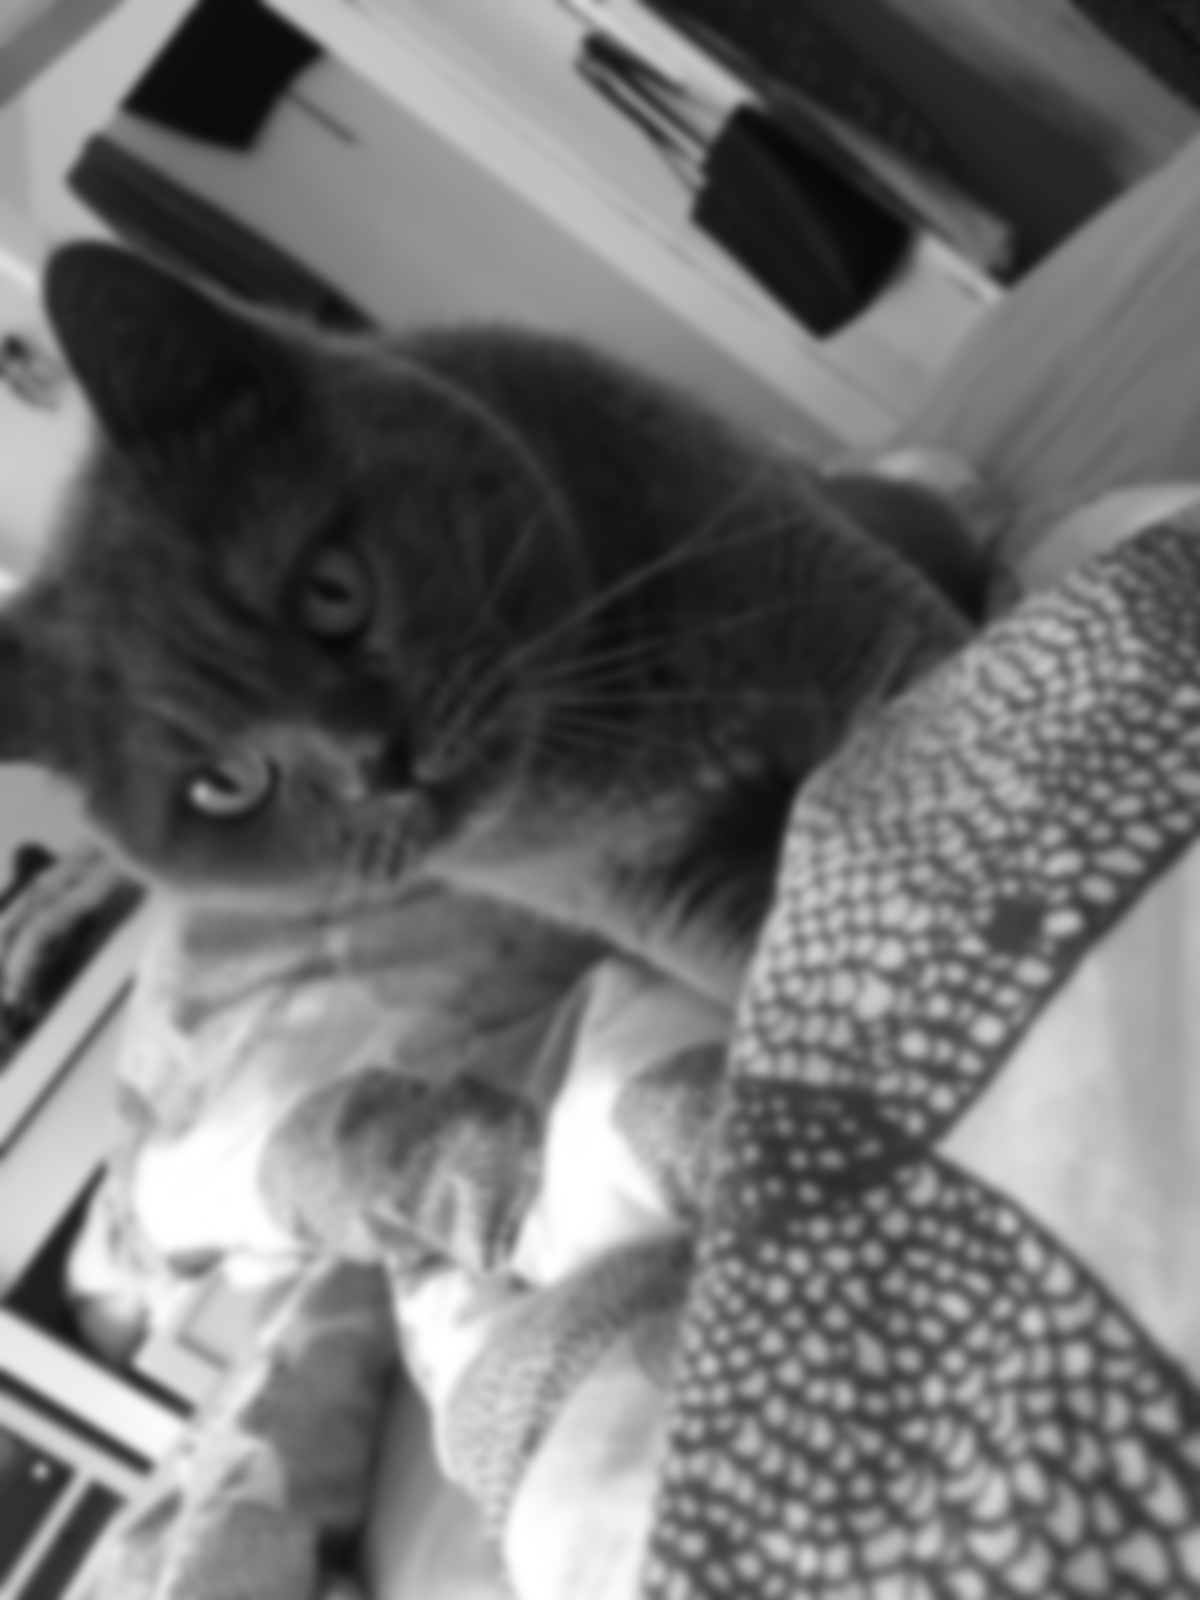
\includegraphics[width=0.4\linewidth]{images/KadseSmooth}
			\caption[Smooth Felix]{Smooth Felix}
			\label{fig:Smooth}
		\end{figure}
	\end{center}
\end{frame}

\begin{frame}
	\frametitle{Problem III: Noise}
	\begin{center}
		\begin{figure}
			\centering
			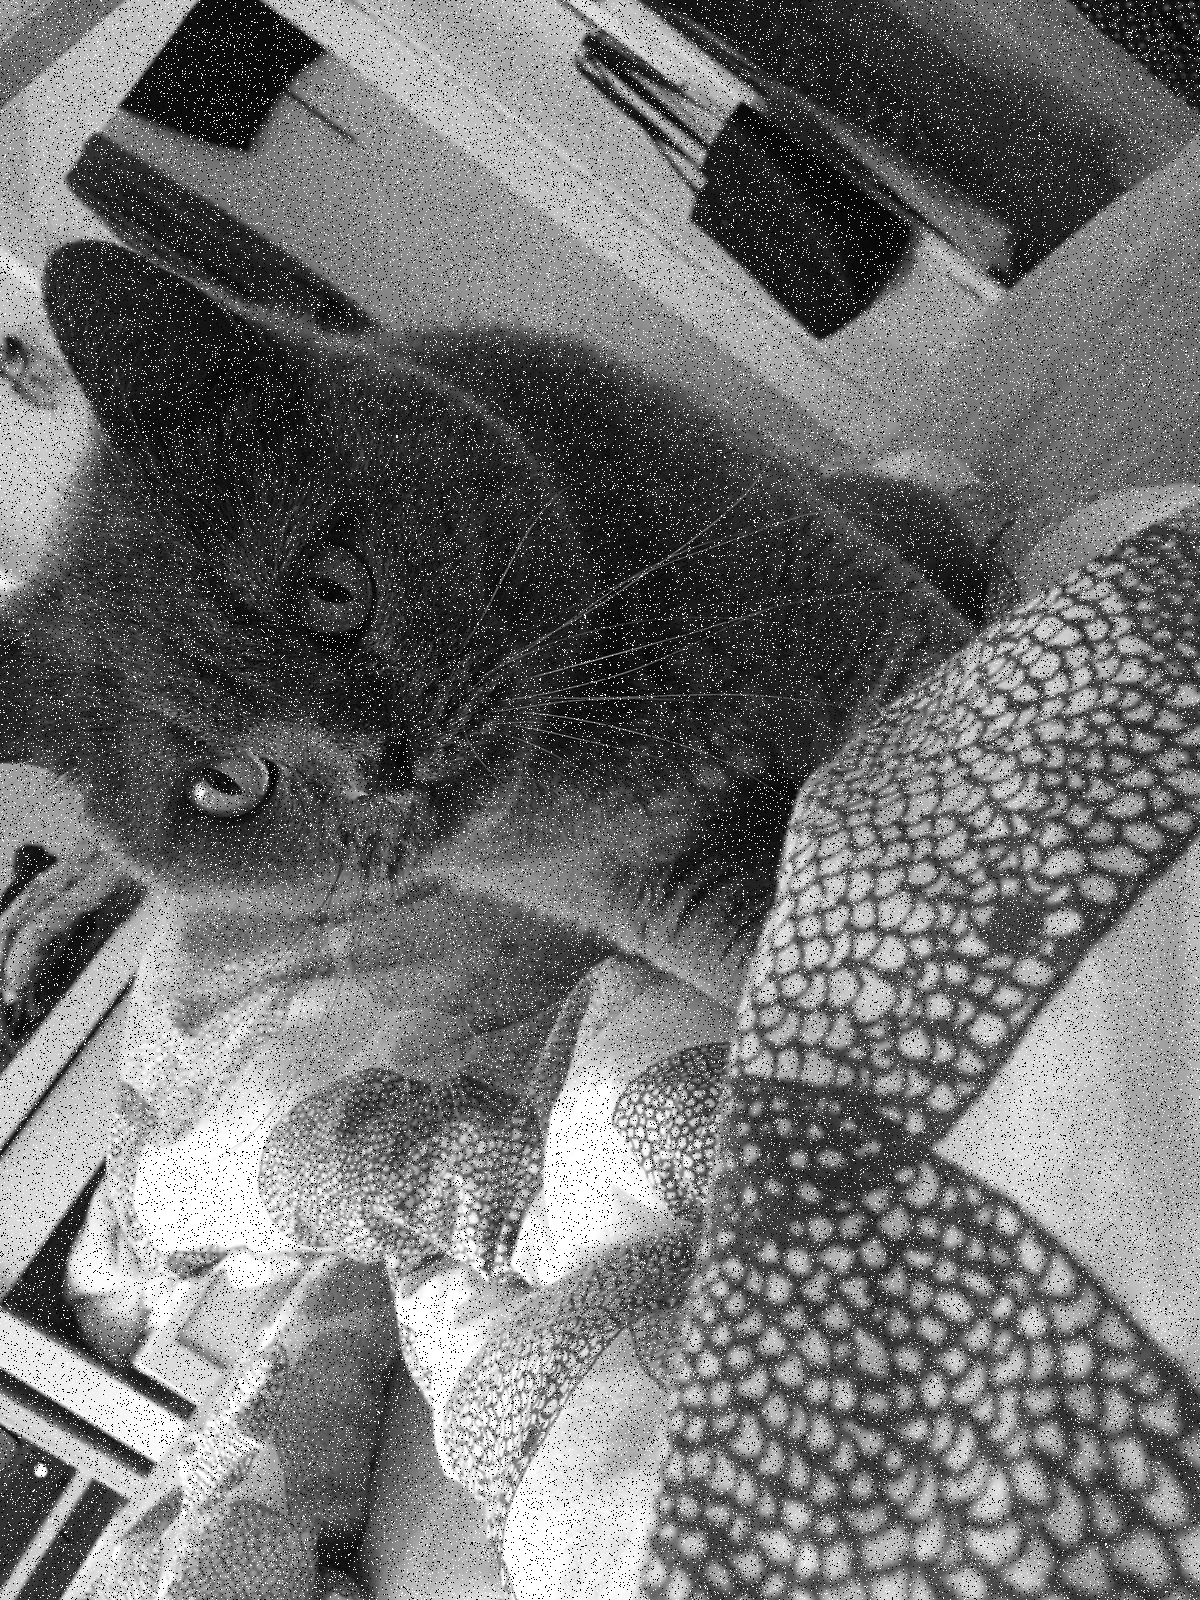
\includegraphics[width=0.4\linewidth]{images/KadseSalty}
			\caption[Salted Felix]{Salted Felix}
			\label{fig:Salted}
		\end{figure}
	\end{center}
\end{frame}

\subsection{Definition}
\begin{frame}
	\frametitle{Definition}
	In Image Processing, an edge can be defined as a set of contiguous pixel positions where an abrupt change of intensity, gray- or color-values occur. Edges represent boundaries between objects and background. Sometimes, the edge-pixel-sequence may be broken due to insufficient intensity difference.(Malay K. Pakhira )
\end{frame}	

\section{Basics of gradient-based edgedetection}
\begin{frame}
	\frametitle{Requirements}
	\begin{enumerate}
		\item color values known (for examples only grayscale)
		\item picture scale known 
		\item loaded as pixelmatrix 
	\end{enumerate}
\end{frame}	

\subsection{1D approach}
\begin{frame}
	\frametitle{One dimensional approach}
	\begin{center}
		\begin{figure}
			\centering
			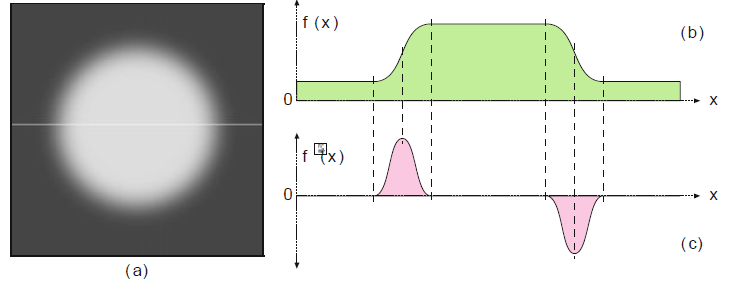
\includegraphics[width=0.7\linewidth]{images/1DGradient}
			\caption[1D Gradient]{One dimensional image function and derivation}
			\label{fig:1dgradient}
		\end{figure}
		\b{Only applyable with known, steady functions}
	\end{center}
\end{frame}

\begin{frame}
	\frametitle{Approximating discrete derivation}
	Problem: the image function is discrete, therefore we need to approximate the derivation
	\begin{center}
		\begin{figure}
			\centering
			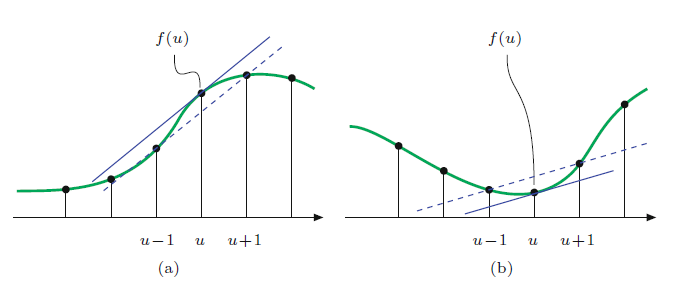
\includegraphics[width=0.7\linewidth]{images/1DGradientApproximation}
			\caption[1D Gradient Approximation]{Approximation of the derivation for discrete imagefunctions}
			\label{fig:1dgradientapprox}
		\end{figure}
		$\dfrac{df}{dx}(u) \approx \dfrac{f(u+1) - f(u-1)}{(u+1)-(u-1)} = \dfrac{f(u+1) - f(u-1)}{2}$
	\end{center}
\end{frame}

\subsection{2D Approach}
\begin{frame}
	\frametitle{Two dimensional approach}
	If working with full images,we got two dimensions and therefore two partial derivations:
	\begin{center}	
		$I_x = \dfrac{\partial I}{\partial x}(u,v) , I_y = \dfrac{\partial I}{\partial y}(u,v)$
	\end{center}
	the \textbf{gradient} at the point \textit{(u,v)} is \newline
	\begin{center}
		$\nabla I(u,v) =  \begin{pmatrix}I_x(u,v) \\ I_y(u,v)\end{pmatrix}$
	\end{center}	
	~\newline
	And the \textbf{magnitude} is \newline
	\begin{center}
		$|\nabla I|=\sqrt{I_x^2 + I_y^2}$
	\end{center}
\end{frame}

\begin{frame}
	\frametitle{Example}
	\begin{figure}
		\centering
		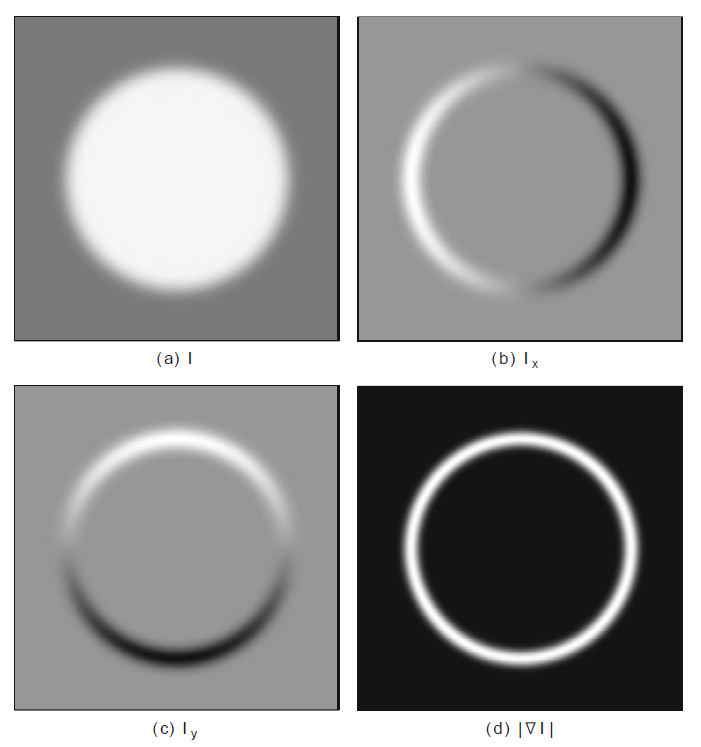
\includegraphics[width=0.5\linewidth]{images/2DEdgeGradient}
		\caption{Visualisation of simple gradient-based edgedetection}
		\label{fig:2dedgegradient}
	\end{figure}
\end{frame}
\subsection{Simple Example}
\begin{frame}
	\frametitle{Example with Felix}
	\begin{figure}
		\centering
		\begin{subfigure}[b]{0.175\textwidth}
			\centering
			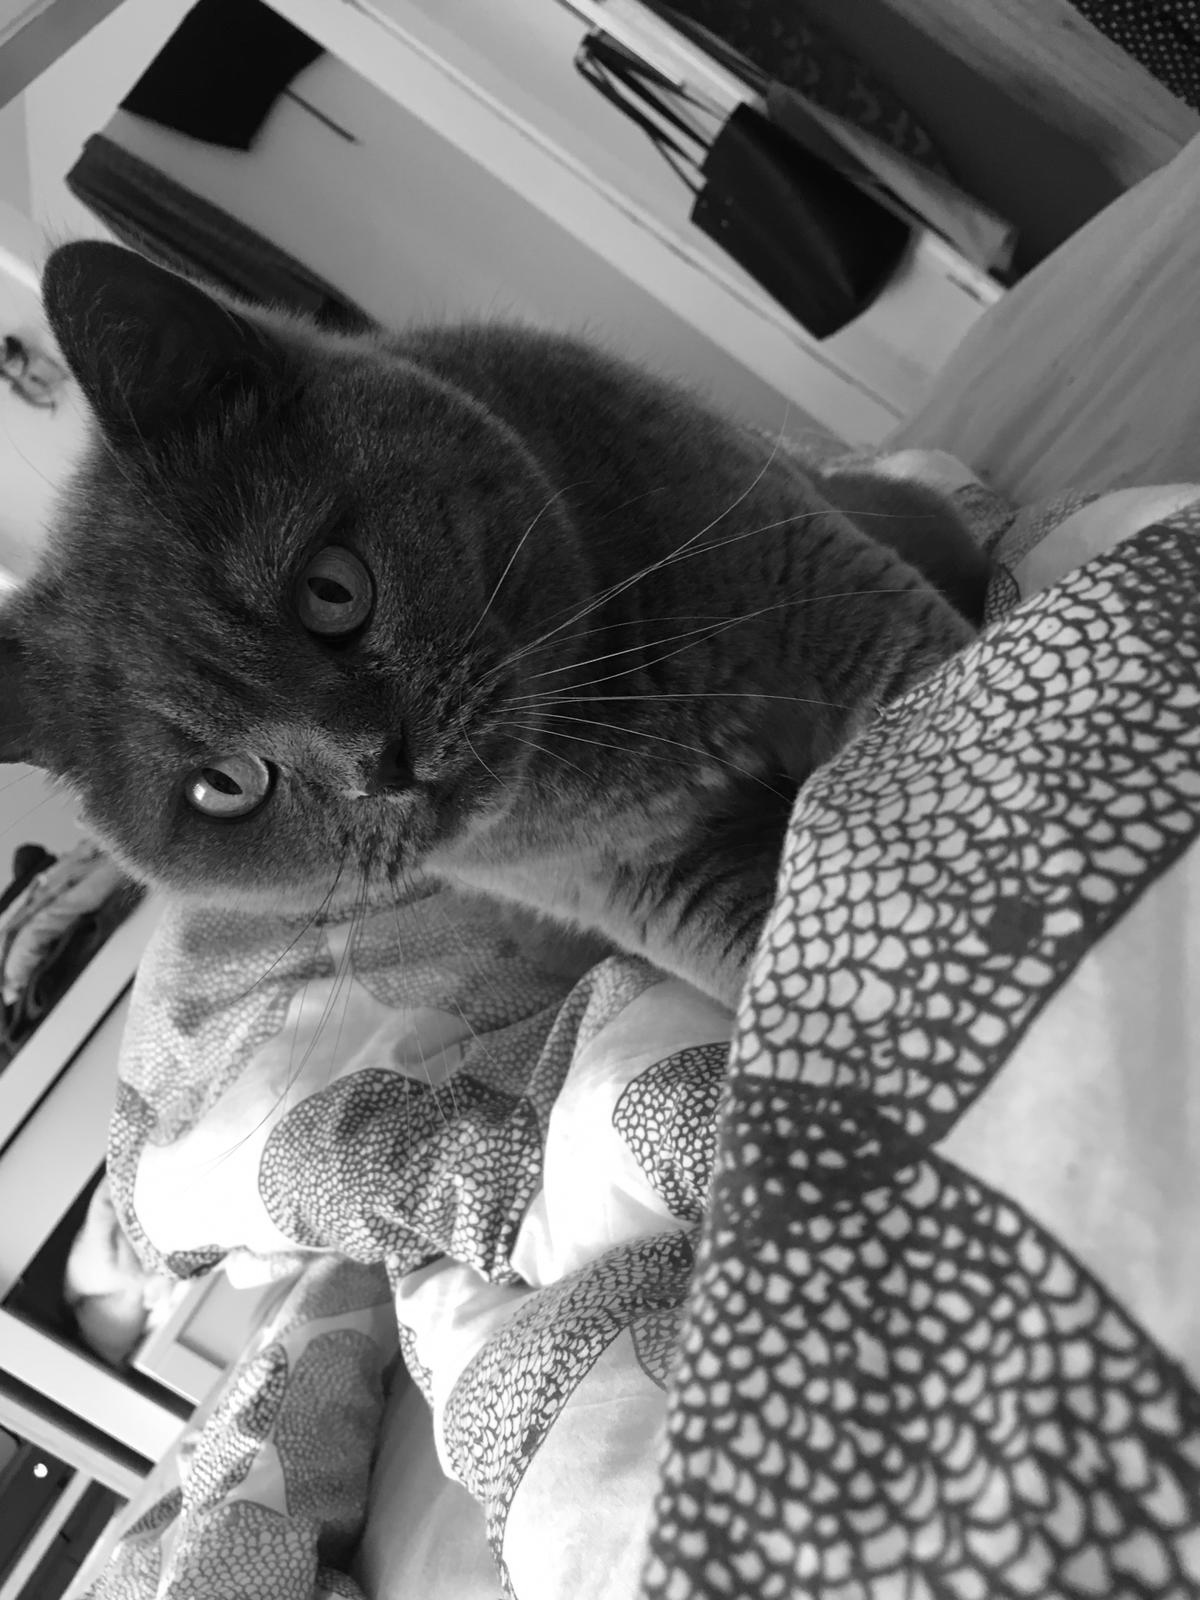
\includegraphics[width=\textwidth]{images/Kadse}
			\caption[I]%
			{{\small I}}    
			\label{fig:RawFelix}
		\end{subfigure}
		\quad
		\begin{subfigure}[b]{0.175\textwidth}  
			\centering 
			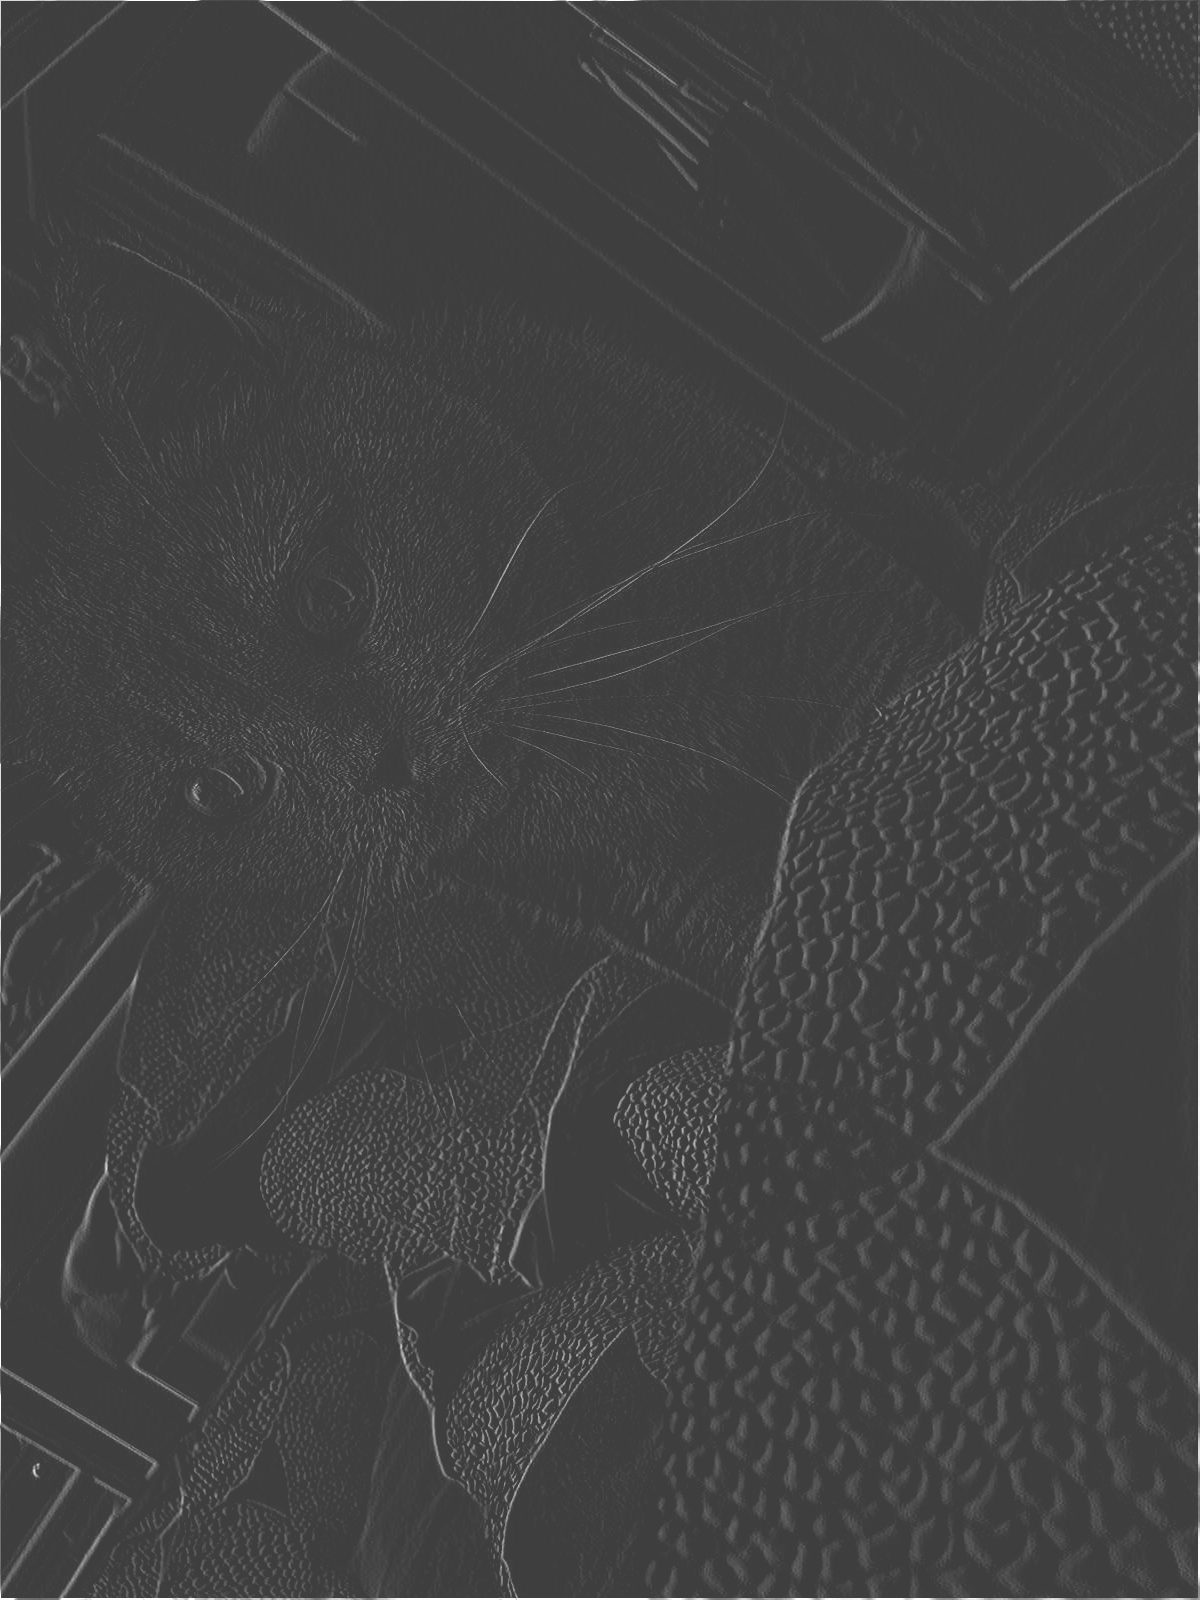
\includegraphics[width=\textwidth]{images/KadseSimpleX}
			\caption[]%
			{{\small $I_x$}}    
			\label{fig:FelixX}
		\end{subfigure}
		\vskip\baselineskip
		\begin{subfigure}[b]{0.175\textwidth}   
			\centering 
			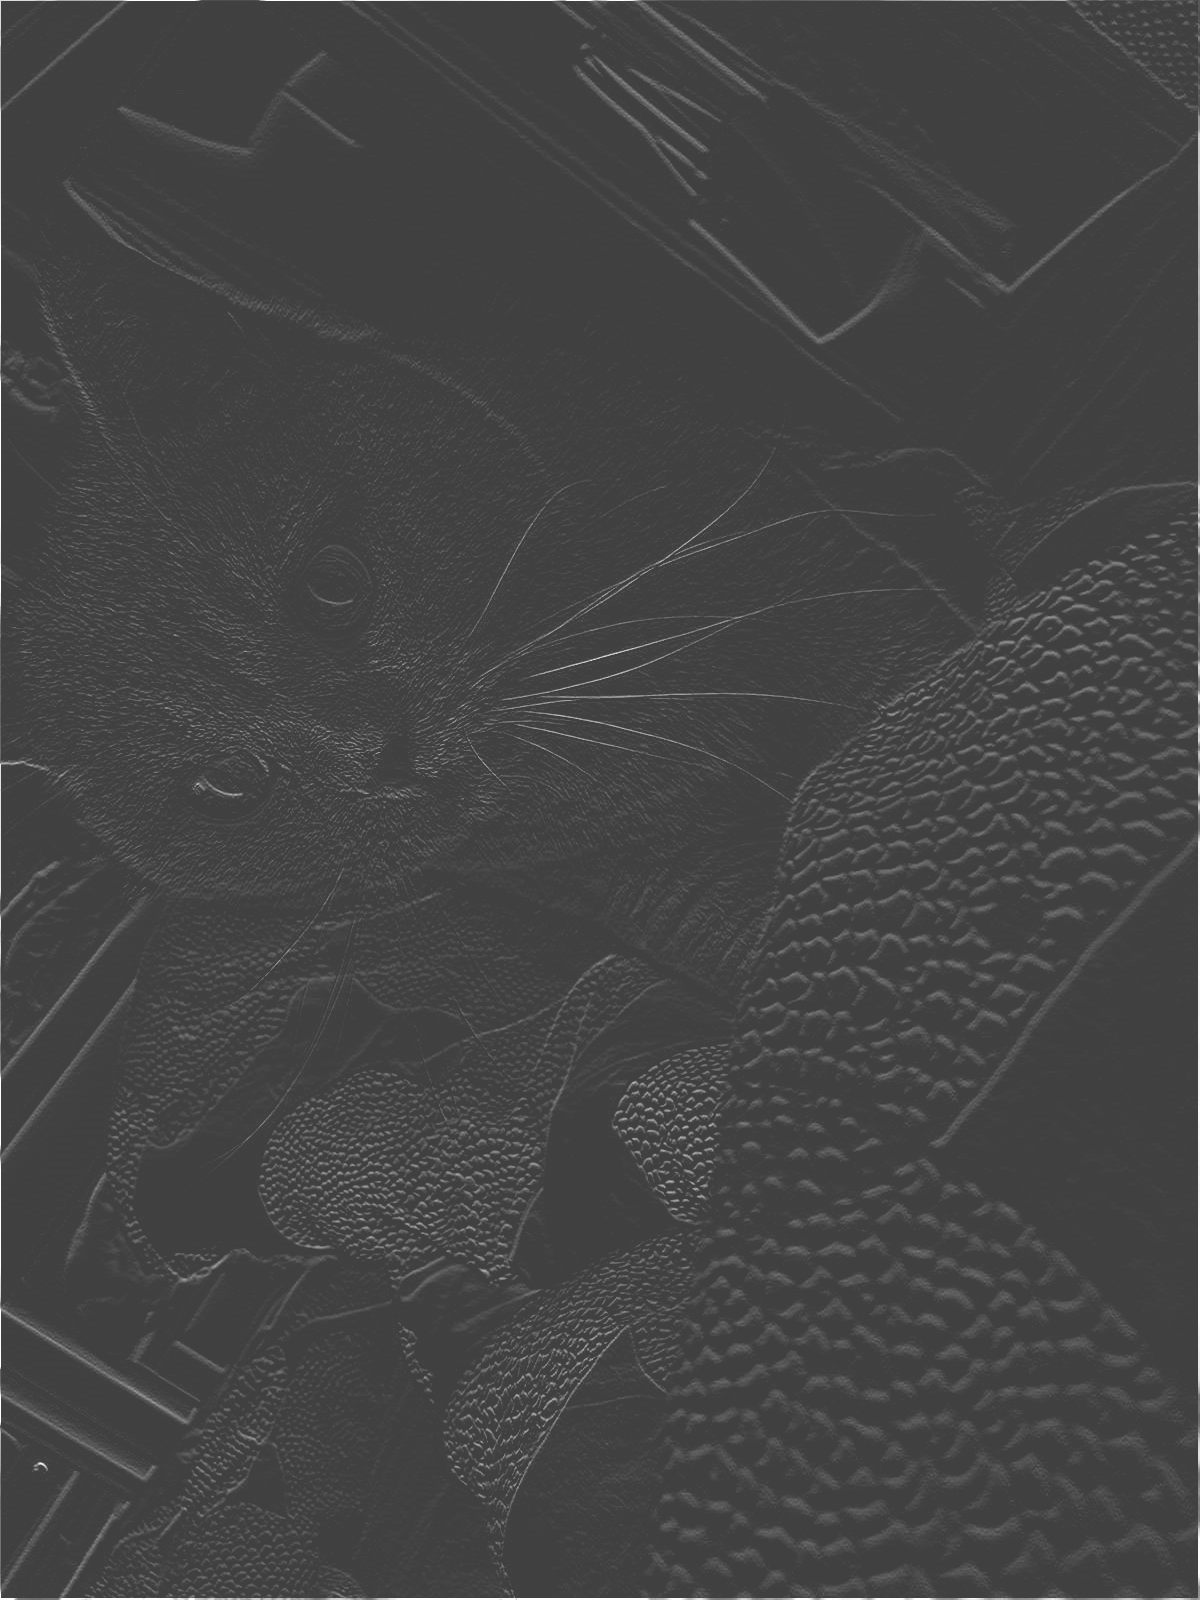
\includegraphics[width=\textwidth]{images/KadseSimpleY}
			\caption[]%
			{{\small $I_y$}}    
			\label{fig:FelixY}
		\end{subfigure}
		\quad
		\begin{subfigure}[b]{0.175\textwidth}   
			\centering 
			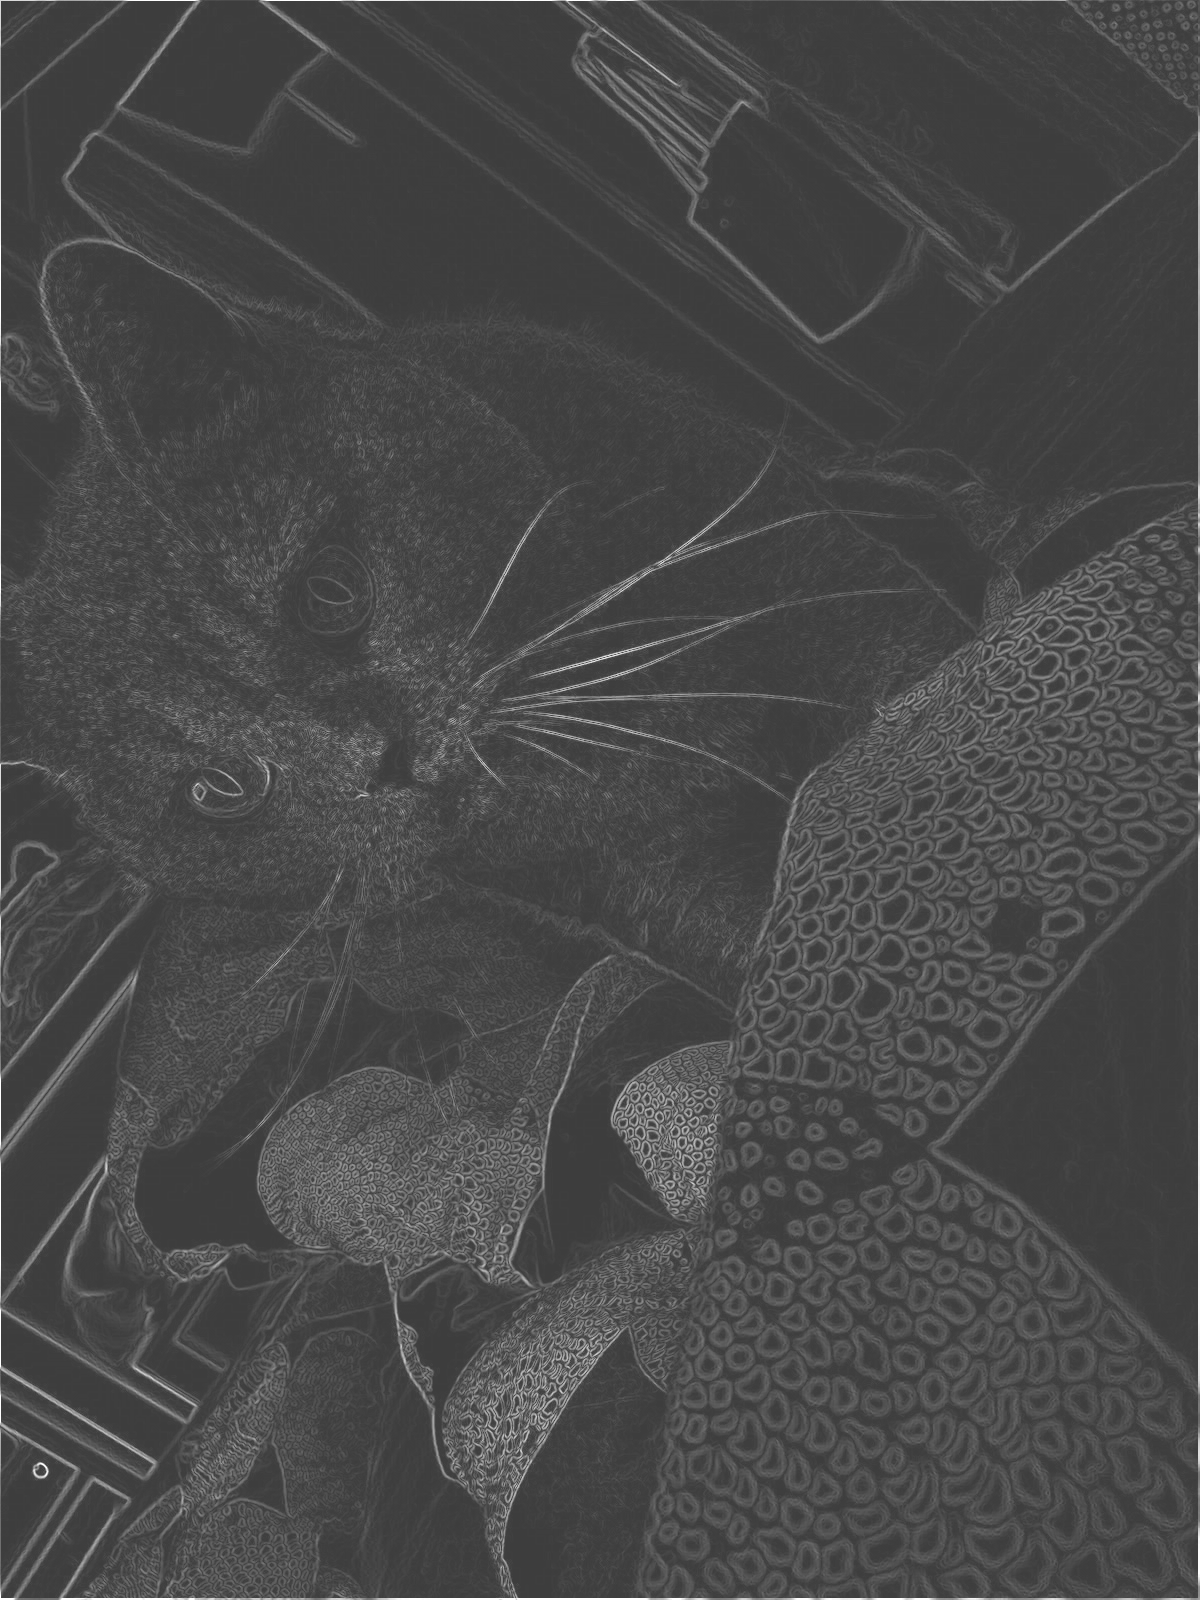
\includegraphics[width=\textwidth]{images/KadseSimple}
			\caption[]%
			{{\small $|\nabla I |$}}    
			\label{fig:FelixSimple}
		\end{subfigure}
		\caption[Simple Filters applied to Felix ]
		{\small Simple Filters applied to Felix\footnote{All images have a 50\% increased brightness}} 
		\label{fig:FullSimpleFelix}
	\end{figure}
	
	
\end{frame}
\subsection{Filters}
\begin{frame}
	\frametitle{Implementation with filters}
	Expressing the gradient as a \textit{linear filter} is simple:
	\begin{columns}
		\begin{column}{0.5\textwidth}
			\begin{center}
				$I_x = \begin{bmatrix} -0.5 & 0 & 0.5\end{bmatrix}$
			\end{center}	
		\end{column}
		\begin{column}{0.5\textwidth} 
			\begin{center}
				$I_y = \begin{bmatrix} -0.5 \\ 0 \\ 0.5\end{bmatrix}$
			\end{center}
		\end{column}
	\end{columns}
\end{frame}

\section{Advanced gradient-based edgedetection}
\subsection{3x3 Filters}
\begin{frame}
	\frametitle{Prewitt Operator}
	\begin{center}
		Idea: Include neighboorhood
	\end{center}
	~\newline
	\begin{columns}
		\begin{column}{0.5\textwidth}
			\begin{center}
				$H^P_x = \begin{bmatrix}
				-1 & 0 & 1 \\ -1 & 0 & 1 \\ -1 & 0 & 1
				\end{bmatrix} $
			\end{center}	
		\end{column}
		\begin{column}{0.5\textwidth} 
			\begin{center}
				$H^P_y = \begin{bmatrix}
				-1 & -1 & -1 \\ 0 & 0 & 0 \\ 1 & 1 & 1
				\end{bmatrix} $
			\end{center}
		\end{column}
	\end{columns}
	~\newline
	\begin{center}
		$\nabla I^P(u,v)\approx \dfrac{1}{6} \cdot \begin{pmatrix}
		(I\ast H^P_x)(u,v) \\ (I\ast H^P_y)(u,v) 
		\end{pmatrix}$
	\end{center}
\end{frame}
\begin{frame}
	\frametitle{Sobel}
	\begin{center}
		Idea: Include neighboorhood but weight center more
	\end{center}
	~\newline	
	\begin{columns}
		\begin{column}{0.5\textwidth}
			\begin{center}
				$H^S_x = \begin{bmatrix}
				-1 & 0 & 1 \\ -2 & 0 & 2 \\ -1 & 0 & 1
				\end{bmatrix} $
			\end{center}	
		\end{column}
		\begin{column}{0.5\textwidth} 
			\begin{center}
				$H^S_y = \begin{bmatrix}
				-1 & -2 & -1 \\ 0 & 0 & 0 \\ 1 & 2 & 1
				\end{bmatrix} $
			\end{center}
		\end{column}
	\end{columns}
	~\newline
	\begin{center}
		$\nabla I^S(u,v)\approx \dfrac{1}{8} \cdot \begin{pmatrix}
		(I\ast H^S_x)(u,v) \\ (I\ast H^S_y)(u,v) 
		\end{pmatrix}$
	\end{center}
\end{frame}
\subsection{3x3 Examples}
\begin{frame}
	\frametitle{Comparison with Felix}
	\begin{columns}
		\begin{column}{0.33\textwidth}
			\begin{figure}
				\centering
				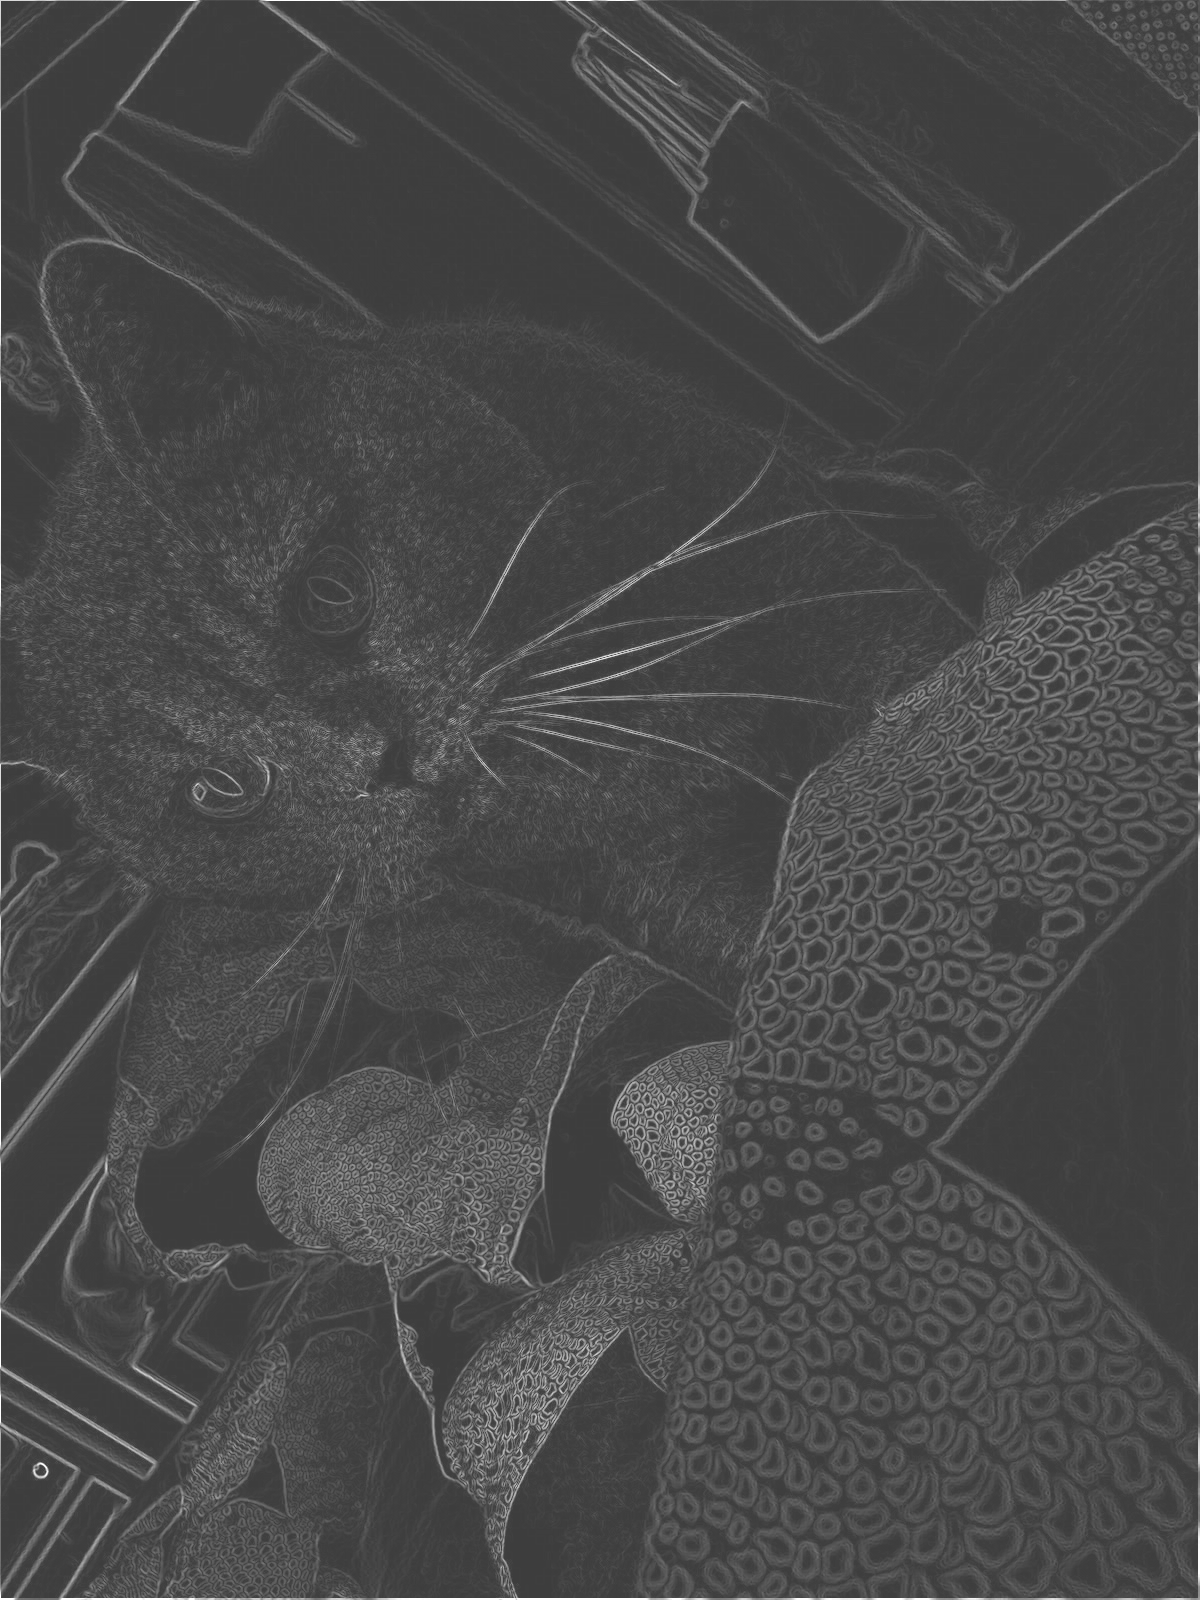
\includegraphics[width=0.8\linewidth]{images/KadseSimple}
				\caption[Simple edge filter]{Simple edge filter}
				\label{fig:Simple}
			\end{figure}
		\end{column}
		\begin{column}{0.33\textwidth}
				\begin{figure}
					\centering
					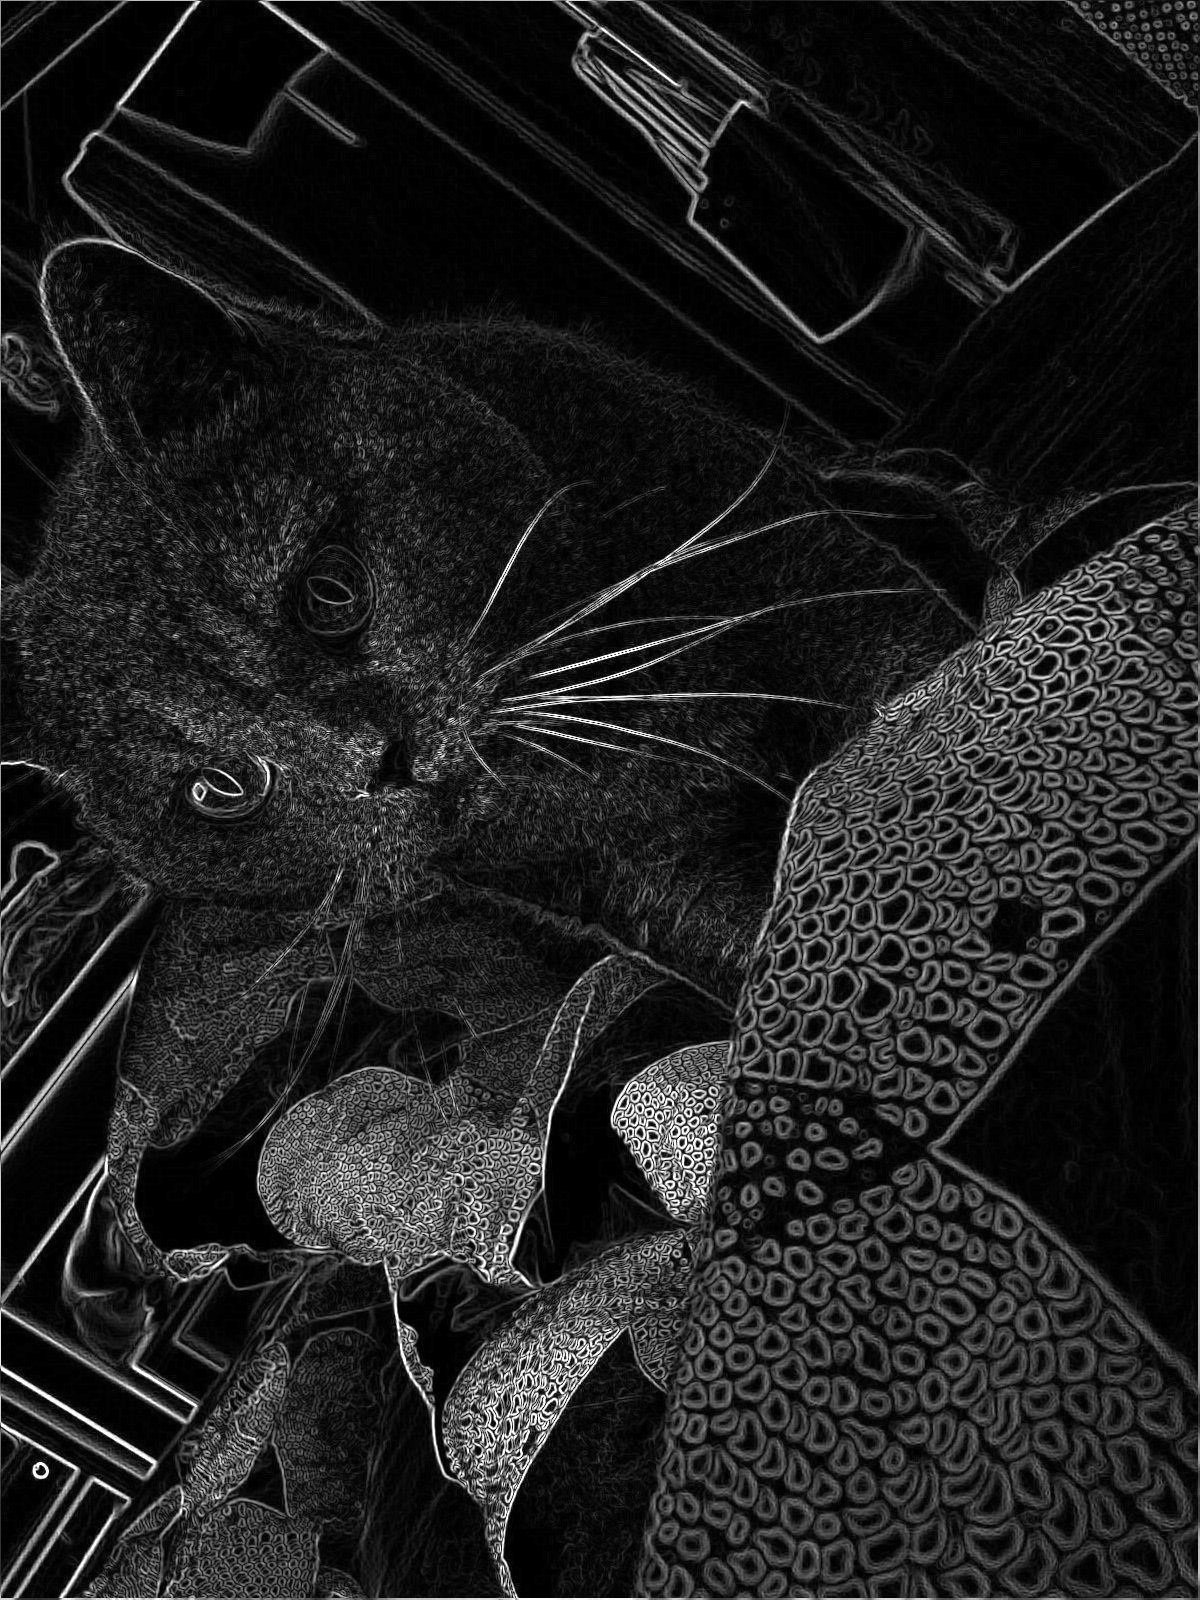
\includegraphics[width=0.8\linewidth]{images/KadsePrewitt}
					\caption[Prewitt Operator]{Prewitt Operator}
					\label{fig:KadsePrewitt}
				\end{figure}
		\end{column}
		\begin{column}{0.33\textwidth}
			\begin{figure}
				\centering
				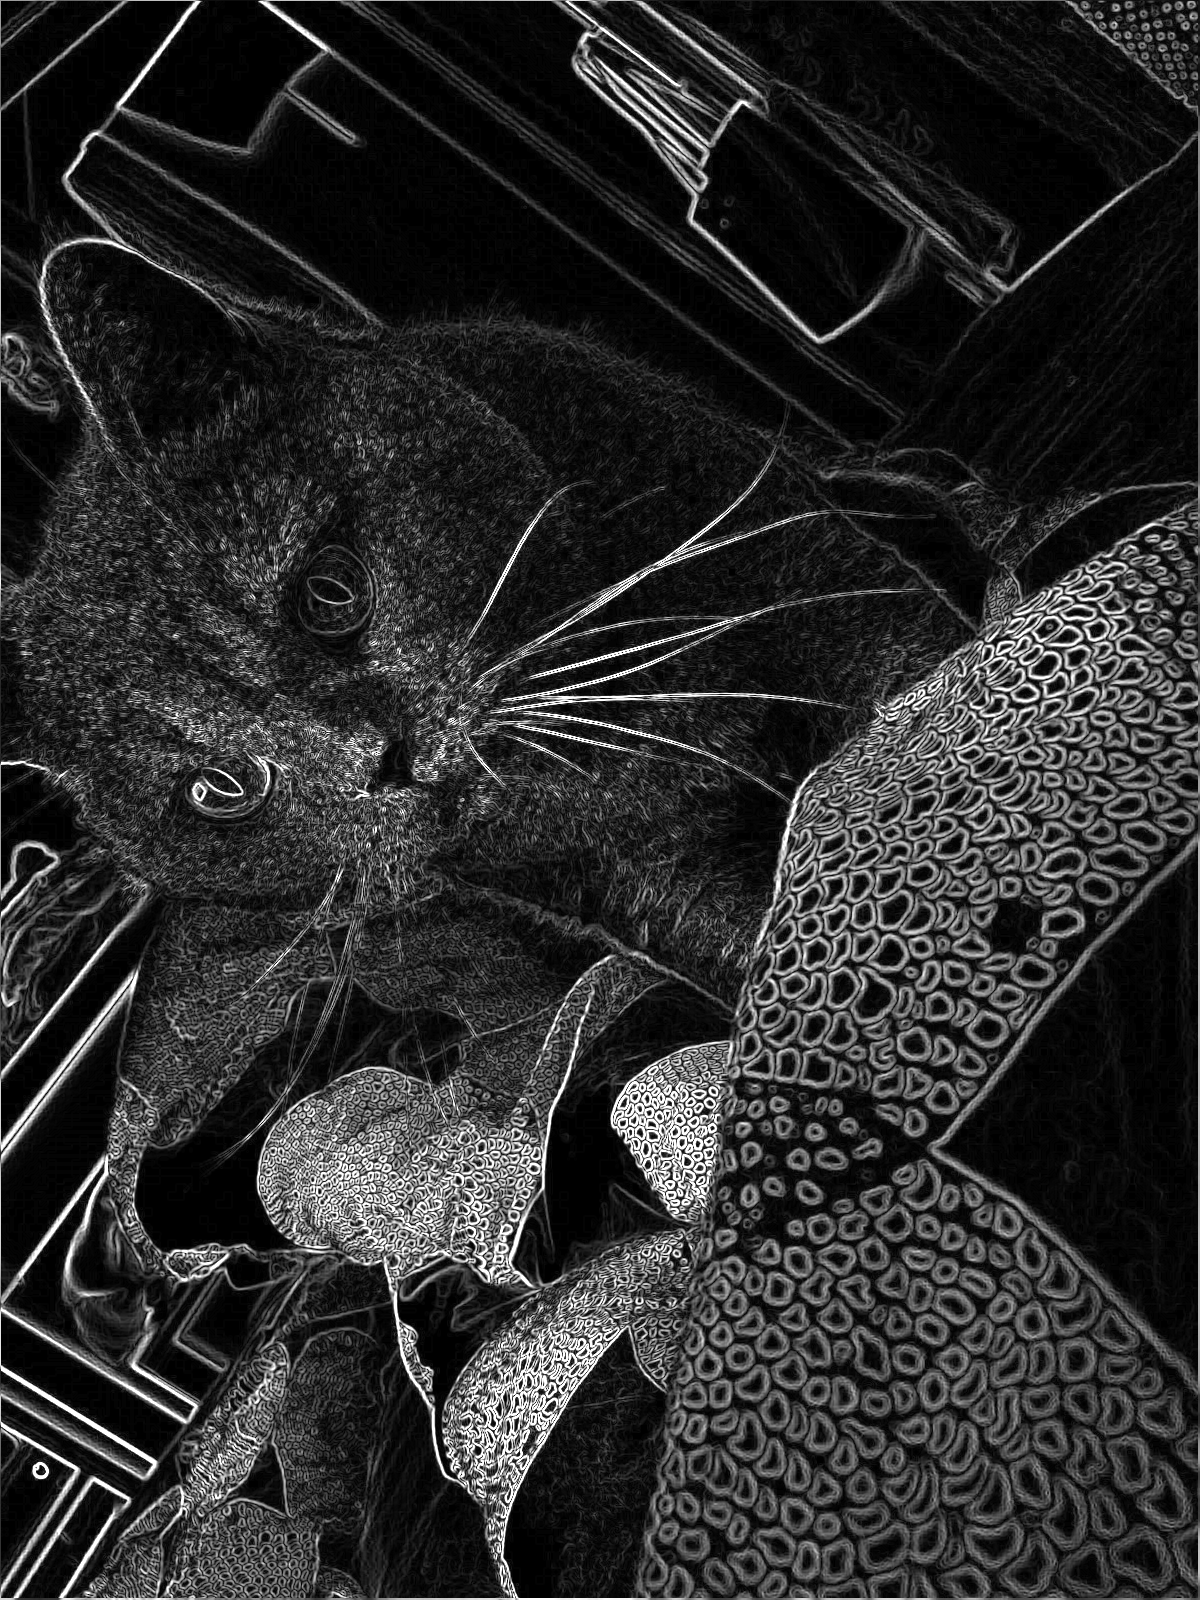
\includegraphics[width=0.8\linewidth]{images/KadseSobel}
				\caption[Sobel Operator]{Sobel Operator}
				\label{fig:KadseSobel}
			\end{figure}
		\end{column}
	\end{columns}
\end{frame}
\subsection{Evaluations}
\begin{frame}
	\frametitle{Evaluations}
	\begin{center}
		\textbf{general magnitude}: $E(u,v) = \sqrt{I_x^2(u,v)+I_y^2(u,v)}$
		\newline holds for every Operator 
		~\newline
		\begin{figure}
			\centering
			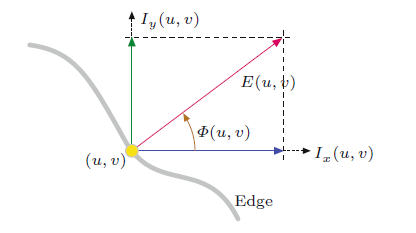
\includegraphics[width=0.5\linewidth]{images/EdgeDirection}
			\caption[Visualisation of edge direction]{Visualisation of edge direction}
			\label{fig:edgedir}
		\end{figure}
		~\newline
		$\Phi(u,v)=\tan^{-1}\left(\dfrac{I_y(u,v)}{I_x(u,v)}\right)=\arctan(I_x(u,v),I_y(u,v))$
	\end{center}
	
\end{frame}
\section{Compass Operators}

\section{Edge Sharpening}

\end{document}